\chapterwithopening{System Design}{chap:system_design}{
  \chaptercontentsitem{sec:system_design_introduction}
  \chaptercontentsitem{sec:architectural_design_overview}
  \chaptercontentsitem{sec:data_and_storage_design}
  \chaptercontentsitem{sec:interface_and_interaction_design}
}

\newcolumntype{L}[1]{>{\raggedright\arraybackslash}p{#1}}

% Reserve space for a heading and the opening of the content that follows it.
\newcommand{\EduNeedspace}[1]{%
  \par
  \begingroup
    \dimen0=#1\relax
    \dimen2=\pagegoal
    \advance\dimen2 by -\pagetotal
    \ifdim\dimen0>\dimen2
      \vfil
      \break
    \fi
  \endgroup
}

\newcommand{\EduSchemaTableStart}[1]{%
  \begingroup
  \footnotesize
  \renewcommand{\arraystretch}{1.14}%
  \setlength{\tabcolsep}{4pt}%
  \begin{longtable}{|L{0.28\textwidth}|L{0.18\textwidth}|L{0.46\textwidth}|}
    \caption{Schema for Table: \db{#1}} \\
    \hline
    \textbf{Column} & \textbf{Type} & \textbf{Attributes} \\
    \hline
    \endfirsthead
    \hline
    \textbf{Column} & \textbf{Type} & \textbf{Attributes} \\
    \hline
    \endhead
    \hline
    \multicolumn{3}{r}{\small\textit{Continued on the next page}} \\
    \endfoot
    \endlastfoot
}

\newcommand{\EduSchemaRow}[3]{%
  \db{#1} & #2 & #3 \\*
  \hline
}

\newcommand{\EduSchemaNote}[1]{%
  \multicolumn{3}{|L{0.92\textwidth}|}{\textit{#1}} \\*
  \hline
}

\newcommand{\EduSchemaTableEnd}{%
  \end{longtable}
  \endgroup
}

\section{Introduction}\label{sec:system_design_introduction}

System design translates the analytical requirements established in the
previous chapter into a structured model for the organization of EduVerse.
This chapter presents the architectural context, information model, relational
database structure, and interface design principles that connect users,
academic workflows, data, and configurable access.

The emphasis is placed on how the major parts of the system are organized and
related at design level, while the technical realization of these decisions is
discussed separately in the implementation chapter.

\section{Design Context and Architectural Structure}\label{sec:architectural_design_overview}

EduVerse is designed as a coordinated educational platform in which related
academic and administrative workflows operate within a shared organizational
and class context. The architecture separates the main user-facing clients
from persistent data, file-handling services, and real-time communication
capabilities while preserving common access and governance rules.

The web application serves as the primary interface for comprehensive academic
and administrative workflows, while the mobile companion extends selected
forms of participation. Persistent academic and organizational data are
managed through the relational data layer, and specialized services support
capabilities such as uploaded learning resources and synchronous sessions.

This structure allows individual services to remain technically distinct while
presenting users with a coherent educational environment governed by shared
organizational, role, class, and feature context.

\section{Information Model and Persistence Design}\label{sec:data_and_storage_design}

The EduVerse information model represents the relationships between
organizations, users, roles, classes, learning resources, assessments,
communication, and configurable platform capabilities. The database design
supports these relationships while preserving the separation between
organization-level governance and class-level academic participation.

This section presents the logical database structure, the Entity Relationship
Diagram (ERD), and the principal schema groups required to support the system
at design level.

\subsection{Logical Database Design}\label{subsec:database_design_overview}

EduVerse uses a relational data model organized around the relationship
between organizations, users, and classes. The organization forms the primary
institutional context, while the class represents the main academic workspace.

Organization membership is separated from class membership so that
institutional roles and class participation can be managed independently. This
distinction supports users who participate in multiple organizations, hold
different roles, or belong to multiple classes.

Academic entities such as materials, communication records, assignments,
examinations, notifications, and live sessions are associated with the relevant
organization and class context. Configuration entities are maintained
separately from ordinary academic content so that feature availability and
institutional settings can be applied without changing the underlying learning
records.

The resulting model supports multi-organization governance, role-aware access,
class participation, academic history, assessment workflows, and configurable
feature availability within one relational structure.

\subsection{Relational Structure Through the ERD}\label{subsec:entity_relationship_diagram}

The Entity Relationship Diagram provides the central design-level
representation of the EduVerse data model. It shows how institutional,
academic, and configuration entities relate to one another and clarifies the
cardinalities that connect users, organizations, classes, learning resources,
assessments, and platform settings.

The model includes direct one-to-many relationships as well as many-to-many
relationships resolved through intermediate membership or configuration
structures. These relationships are important because users may participate in
multiple organizational and academic contexts rather than belonging to one
fixed system role or class.

\newpage

\paragraph*{Principal Relationship Structure}

\begin{itemize}
  \item \textbf{Organization and membership structure.}
    Organizations provide the institutional context for memberships, classes,
    settings, invitations, and configurable capabilities. User membership
    records connect individual accounts to the organizations in which they
    participate.

  \item \textbf{Role structure.}
    Membership and role relationships allow access responsibilities to be
    represented within an organization context rather than assigning one
    permanent platform-wide role to each user.

  \item \textbf{Class participation structure.}
    Classes belong to organizations, while class-membership relationships
    connect users to the academic workspaces in which they participate. This
    resolves the many-to-many relationship between users and classes.

  \item \textbf{Learning and communication structure.}
    Materials and communication records are associated with classes so that
    learning resources and class interaction remain tied to the appropriate
    academic context.

  \item \textbf{Assessment structure.}
    Classes contain assignments and examinations, with related submission,
    question, attempt, and answer records representing the main assessment
    relationships.

  \item \textbf{Configuration structure.}
    Feature and extension settings relate platform capabilities to organization
    and class contexts, allowing supported tools to vary without changing the
    core academic data model.
\end{itemize}

\paragraph*{Design Significance}

The relational structure separates institutional membership, class
participation, academic content, assessment, and feature configuration while
preserving the relationships required between them. Intermediate membership
and configuration entities are particularly important because several
EduVerse relationships depend on context rather than simple ownership.

The ERD therefore provides the main design-level view of how organizational
governance and academic activity are represented within the same data model.

\begin{figure}[p]
  \centering
  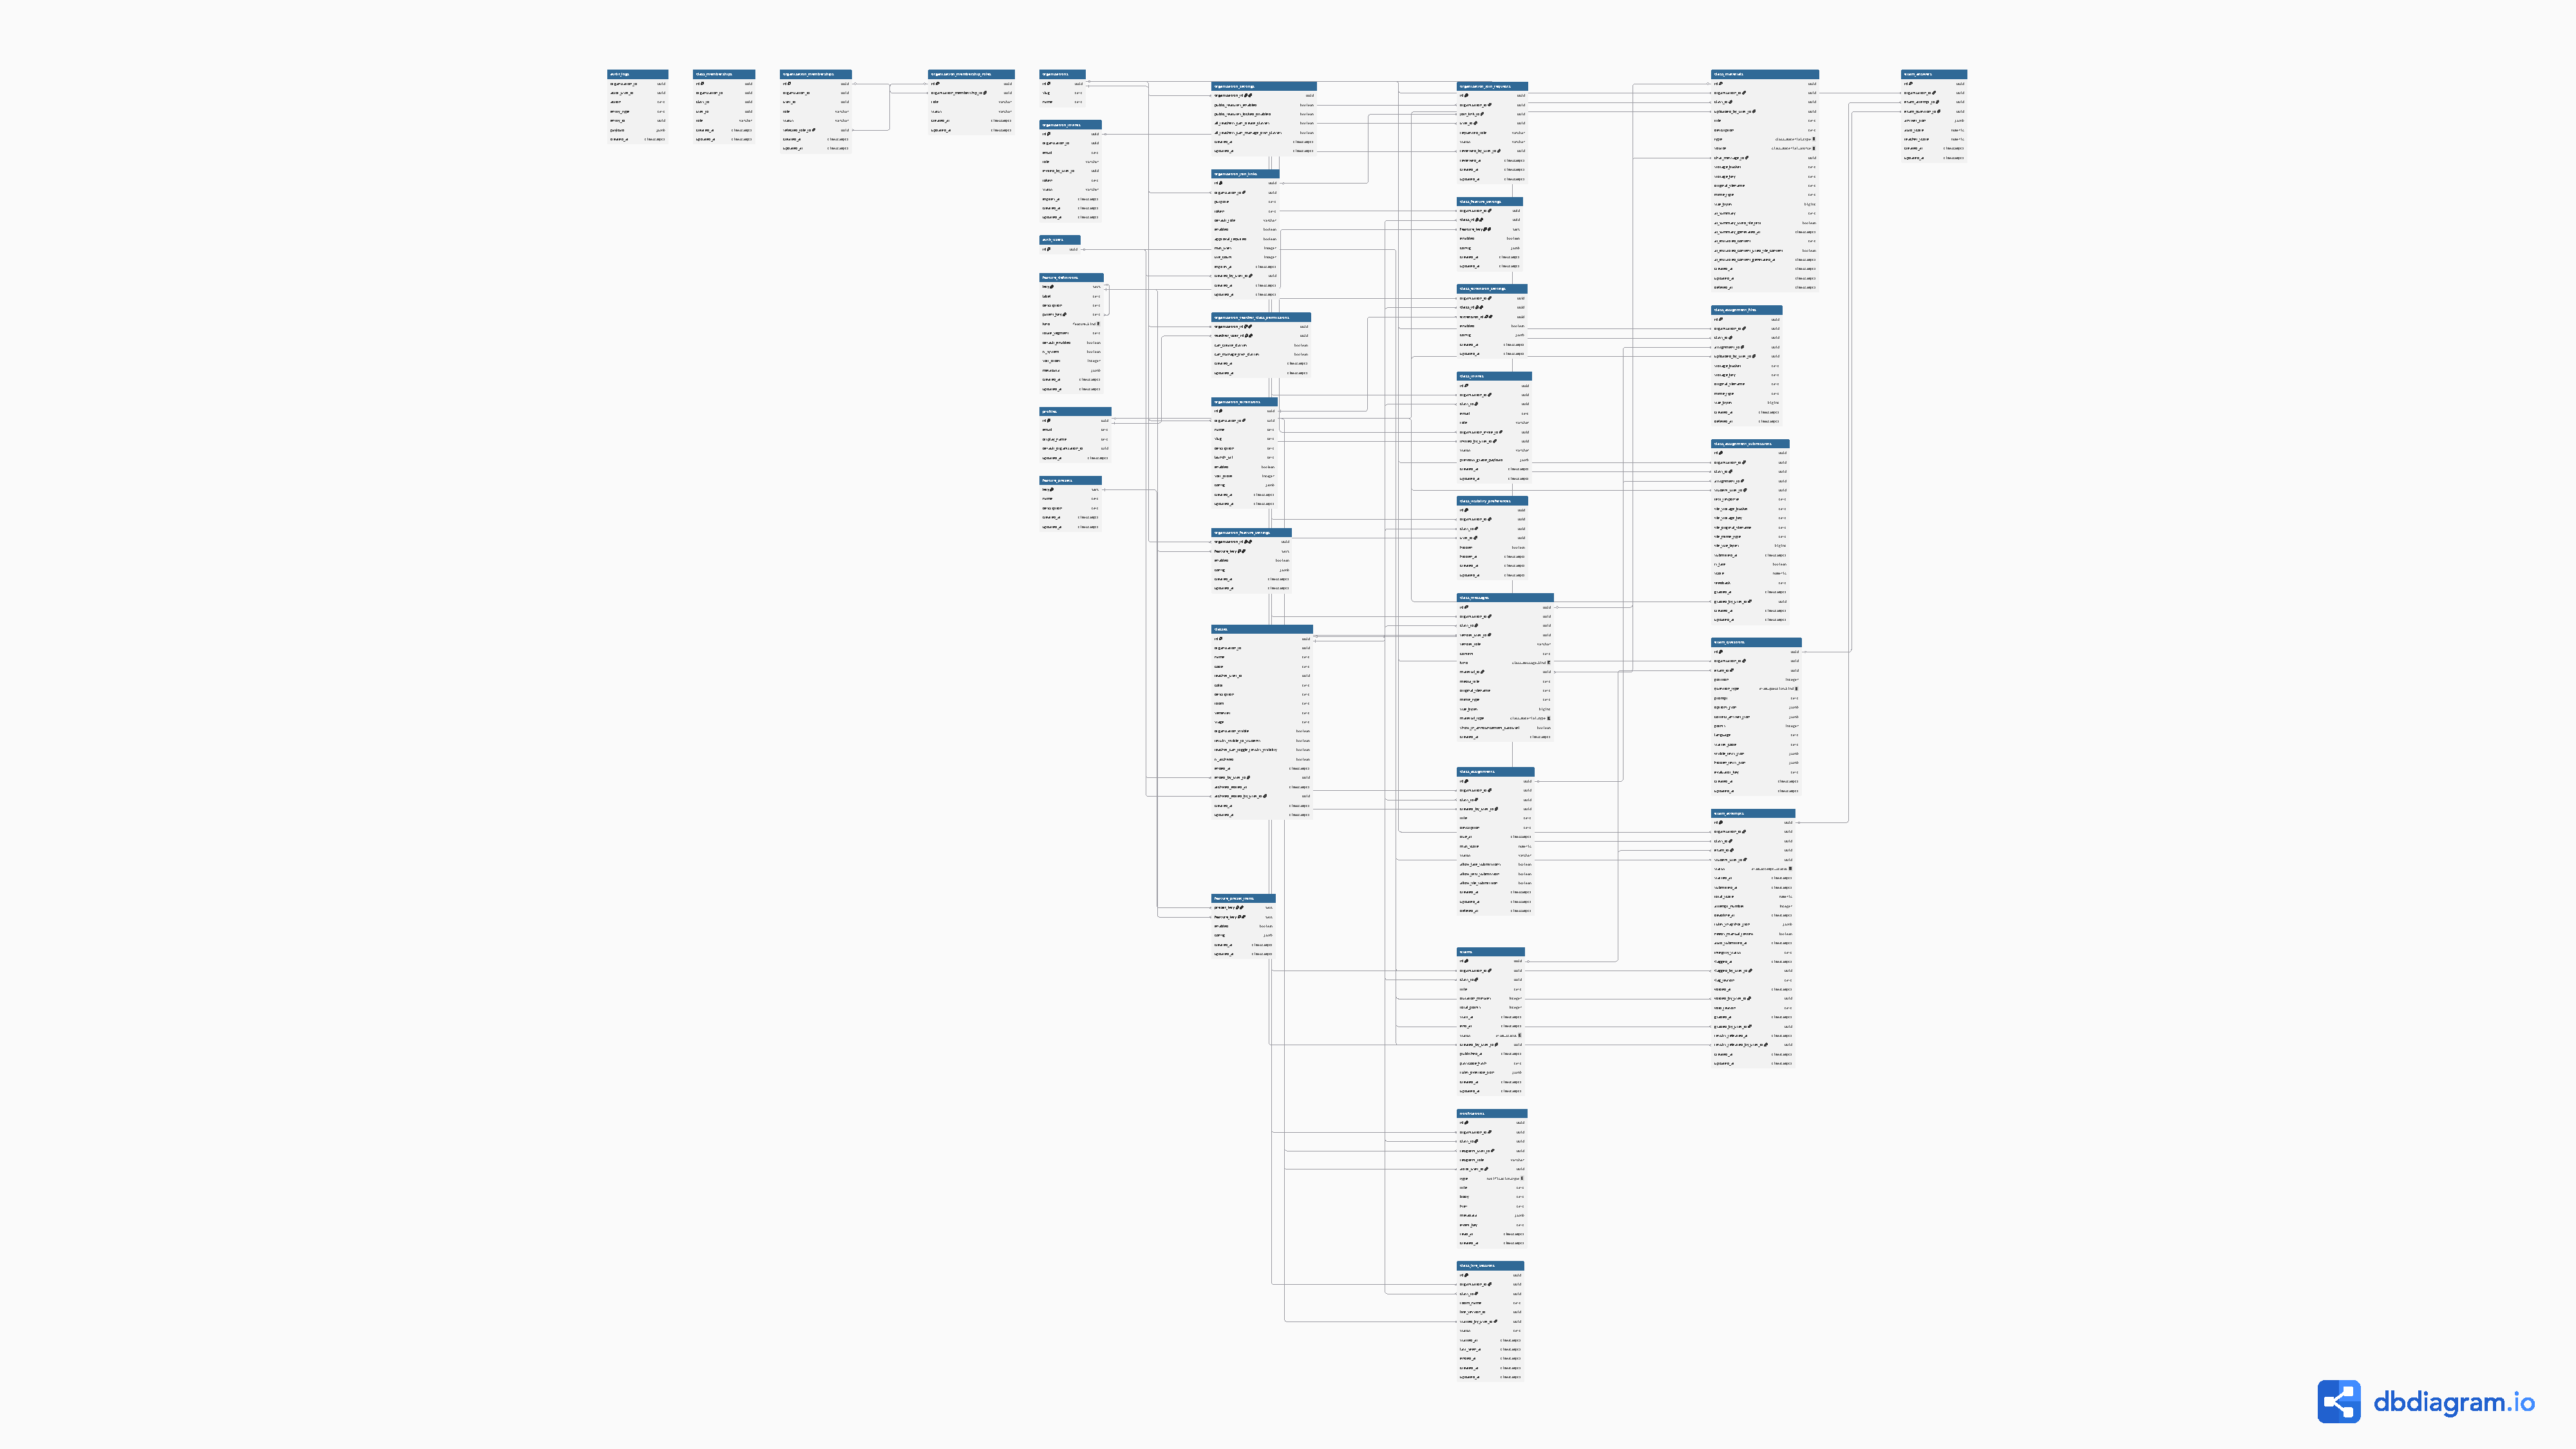
\includegraphics[
    page=1,
    angle=0,
    trim=580 25 580 25,
    clip,
    width=0.97\textwidth,
    height=0.93\textheight,
    keepaspectratio
  ]{figures/chapter5/database-erd.pdf}
  \caption{Entity Relationship Diagram of the EduVerse Database}
  \label{fig:eduverse_database_erd}
\end{figure}

\clearpage

\subsection{Principal Schema Groups}\label{subsec:principal_schema_groups}

The relational model is organized into several schema groups that correspond
to the main institutional and academic responsibilities of EduVerse. The
following overview introduces the principal table groups and their design
purpose before the detailed physical schema documentation.

\begingroup
\footnotesize
\renewcommand{\arraystretch}{1.16}
\setlength{\tabcolsep}{3pt}
\begin{longtable}{|L{0.18\textwidth}|L{0.35\textwidth}|L{0.39\textwidth}|}
  \caption{Principal Schema Groups in EduVerse}
  \label{tab:principal_schema_groups} \\
  \hline
  \textbf{Schema Group} & \textbf{Principal Tables} & \textbf{Design Purpose} \\
  \hline
  \endfirsthead
  \hline
  \textbf{Schema Group} & \textbf{Principal Tables} & \textbf{Design Purpose} \\
  \hline
  \endhead
  \hline
  \multicolumn{3}{r}{\small\textit{Continued on the next page}} \\
  \endfoot
  \hline
  \endlastfoot

  Core Organization and Identity &
  \db{organizations}, \db{profiles}, \db{organization_memberships},
  \db{organization_membership_roles} &
  Represents institutional workspaces, user identity context, organization
  membership, and role relationships. \\
  \hline

  Organization Access and Governance &
  \db{organization_invites}, \db{organization_settings},
  \db{organization_teacher_class_permissions}, \db{organization_join_links},
  \db{organization_join_requests} &
  Supports controlled membership entry, administrative settings, teacher
  permissions, and organization-level access governance. \\
  \hline

  Classes and Participation &
  \db{classes}, \db{class_memberships}, \db{class_visibility_preferences},
  \db{class_invites} &
  Represents class workspaces, participation, visibility, membership, and class
  lifecycle relationships. \\
  \hline

  Features and Extensions &
  \db{feature_definitions}, \db{feature_presets},
  \db{feature_preset_items}, \db{organization_feature_settings},
  \db{class_feature_settings}, \db{organization_extensions},
  \db{class_extension_settings} &
  Represents configurable platform capabilities and their organization- or
  class-level availability. \\
  \hline

  Materials and Communication &
  \db{class_materials}, \db{class_messages}, \db{notifications} &
  Supports class learning resources, communication, announcements, and user
  notification records. \\
  \hline

  Assignments and Submissions &
  \db{class_assignments}, \db{class_assignment_files},
  \db{class_assignment_submissions} &
  Represents assignment authoring, attached resources, student submission,
  grading, and feedback relationships. \\
  \hline

  Examinations &
  \db{exams}, \db{exam_questions}, \db{exam_attempts}, \db{exam_answers} &
  Represents examination definition, questions, student attempts, answers,
  grading, and assessment-state relationships. \\
  \hline

  Live Learning &
  \db{class_live_sessions} &
  Represents the lifecycle and class association of synchronous learning
  sessions. \\
  \hline

  System Audit &
  \db{audit_logs} &
  Represents recorded platform actions used for governance, traceability, and
  workflow history. \\
\end{longtable}
\endgroup

\subsection{Physical Schema Tables}
\label{subsec:database_tables}

The following tables document the principal columns, data types, keys, and
relationships of the EduVerse database. Table and column names are preserved
exactly as they appear in the documented schema.

\subsubsection*{Core Multi-Organization and User Model}

\EduSchemaTableStart{organizations}
\EduSchemaRow{id}{\db{uuid}}{PK.}
\EduSchemaRow{slug}{\db{text}}{Organization slug.}
\EduSchemaRow{name}{\db{text}}{Organization display name.}
\EduSchemaTableEnd

\EduSchemaTableStart{profiles}
\EduSchemaRow{id}{\db{uuid}}{PK; aligned with \db{auth.users.id} in the identity model.}
\EduSchemaRow{email}{\db{text}}{Profile email address.}
\EduSchemaRow{display_name}{\db{text}}{Visible user name.}
\EduSchemaRow{default_organization_id}{\db{uuid}}{Related to \db{organizations.id}.}
\EduSchemaRow{updated_at}{\db{timestamp}}{Profile update timestamp.}
\EduSchemaTableEnd

\subsubsection*{Roles, Memberships, Invitations, and Public Join Access}

\EduSchemaTableStart{organization_memberships}
\EduSchemaRow{id}{\db{uuid}}{PK.}
\EduSchemaRow{organization_id}{\db{uuid}}{Related to \db{organizations.id}.}
\EduSchemaRow{user_id}{\db{uuid}}{Related to the profile or authentication identity.}
\EduSchemaRow{role}{\db{public.app_role}}{Role enum.}
\EduSchemaRow{status}{\db{public.membership_status}}{Membership status enum.}
\EduSchemaRow{selected_role_id}{\db{uuid}}{\db{FK to organization_membership_roles.id}.}
\EduSchemaRow{created_at}{\db{timestamp}}{Creation timestamp.}
\EduSchemaRow{updated_at}{\db{timestamp}}{Update timestamp.}
\EduSchemaTableEnd

\EduSchemaTableStart{organization_membership_roles}
\EduSchemaRow{id}{\db{uuid}}{PK.}
\EduSchemaRow{organization_membership_id}{\db{uuid}}{\db{FK to organization_memberships.id}.}
\EduSchemaRow{role}{\db{public.app_role}}{Role enum.}
\EduSchemaRow{status}{\db{public.membership_status}}{Membership status enum.}
\EduSchemaRow{created_at}{\db{timestamp}}{Creation timestamp.}
\EduSchemaRow{updated_at}{\db{timestamp}}{Update timestamp.}
\EduSchemaTableEnd

\EduSchemaTableStart{organization_invites}
\EduSchemaRow{id}{\db{uuid}}{PK.}
\EduSchemaRow{organization_id}{\db{uuid}}{Related to \db{organizations.id}.}
\EduSchemaRow{email}{\db{text}}{Invite target email.}
\EduSchemaRow{role}{\db{public.app_role}}{Role enum.}
\EduSchemaRow{invited_by_user_id}{\db{uuid}}{Related to \db{auth.users.id}.}
\EduSchemaRow{token}{\db{text}}{Invite token.}
\EduSchemaRow{status}{\db{text}}{Invitation-status field used in the organization invite workflow.}
\EduSchemaRow{expires_at}{\db{timestamp}}{Invite expiry timestamp.}
\EduSchemaRow{created_at}{\db{timestamp}}{Creation timestamp.}
\EduSchemaRow{updated_at}{\db{timestamp}}{Update timestamp.}
\EduSchemaTableEnd

\EduSchemaTableStart{organization_settings}
\EduSchemaRow{organization_id}{\db{uuid}}{PK; \db{FK to organizations.id}.}
\EduSchemaRow{public_features_enabled}{\db{boolean}}{Public-feature availability flag.}
\EduSchemaRow{public_features_locked_disabled}{\db{boolean}}{Preset lock flag for disabled public features.}
\EduSchemaRow{all_teachers_can_create_classes}{\db{boolean}}{Teacher class-creation permission flag.}
\EduSchemaRow{all_teachers_can_manage_own_classes}{\db{boolean}}{Teacher class self-management permission flag.}
\EduSchemaRow{created_at}{\db{timestamp}}{Creation timestamp.}
\EduSchemaRow{updated_at}{\db{timestamp}}{Update timestamp.}
\EduSchemaTableEnd

\EduSchemaTableStart{organization_teacher_class_permissions}
\EduSchemaRow{organization_id}{\db{uuid}}{Composite PK; \db{FK to organizations.id}.}
\EduSchemaRow{teacher_user_id}{\db{uuid}}{Composite PK; \db{FK to profiles.id}.}
\EduSchemaRow{can_create_classes}{\db{boolean}}{Teacher override flag for class creation.}
\EduSchemaRow{can_manage_own_classes}{\db{boolean}}{Teacher override flag for managing owned classes.}
\EduSchemaRow{created_at}{\db{timestamp}}{Creation timestamp.}
\EduSchemaRow{updated_at}{\db{timestamp}}{Update timestamp.}
\EduSchemaTableEnd

\EduSchemaTableStart{organization_join_links}
\EduSchemaRow{id}{\db{uuid}}{PK.}
\EduSchemaRow{organization_id}{\db{uuid}}{\db{FK to organizations.id}.}
\EduSchemaRow{purpose}{\db{text}}{Join-link purpose descriptor.}
\EduSchemaRow{token}{\db{text}}{Join token.}
\EduSchemaRow{default_role}{\db{public.app_role}}{Default role enum, constrained to teacher or student.}
\EduSchemaRow{enabled}{\db{boolean}}{Link availability flag.}
\EduSchemaRow{approval_required}{\db{boolean}}{Approval workflow flag.}
\EduSchemaRow{max_uses}{\db{integer}}{Optional usage limit.}
\EduSchemaRow{use_count}{\db{integer}}{Current usage counter.}
\EduSchemaRow{expires_at}{\db{timestamp}}{Link expiry timestamp.}
\EduSchemaRow{created_by_user_id}{\db{uuid}}{\db{FK to auth.users.id}.}
\EduSchemaRow{created_at}{\db{timestamp}}{Creation timestamp.}
\EduSchemaRow{updated_at}{\db{timestamp}}{Update timestamp.}
\EduSchemaTableEnd

\EduSchemaTableStart{organization_join_requests}
\EduSchemaRow{id}{\db{uuid}}{PK.}
\EduSchemaRow{organization_id}{\db{uuid}}{\db{FK to organizations.id}.}
\EduSchemaRow{join_link_id}{\db{uuid}}{\db{FK to organization_join_links.id}.}
\EduSchemaRow{user_id}{\db{uuid}}{\db{FK to auth.users.id}.}
\EduSchemaRow{requested_role}{\db{public.app_role}}{Requested role enum.}
\EduSchemaRow{status}{\db{text}}{Status text; current values include \db{pending}, \db{approved}, and \db{rejected}.}
\EduSchemaRow{reviewed_by_user_id}{\db{uuid}}{\db{FK to auth.users.id}.}
\EduSchemaRow{reviewed_at}{\db{timestamp}}{Review timestamp.}
\EduSchemaRow{created_at}{\db{timestamp}}{Creation timestamp.}
\EduSchemaRow{updated_at}{\db{timestamp}}{Update timestamp.}
\EduSchemaTableEnd

\EduSchemaTableStart{class_invites}
\EduSchemaRow{id}{\db{uuid}}{PK.}
\EduSchemaRow{organization_id}{\db{uuid}}{\db{FK to organizations.id}.}
\EduSchemaRow{class_id}{\db{uuid}}{\db{FK to classes.id}.}
\EduSchemaRow{email}{\db{text}}{Invite target email.}
\EduSchemaRow{role}{\db{public.class_membership_role}}{Class membership role enum.}
\EduSchemaRow{organization_invite_id}{\db{uuid}}{\db{FK to organization_invites.id}.}
\EduSchemaRow{invited_by_user_id}{\db{uuid}}{\db{FK to auth.users.id}.}
\EduSchemaRow{status}{\db{public.membership_status}}{Membership status enum.}
\EduSchemaRow{previous_grade_payload}{\db{json/jsonb}}{Imported previous-term grade payload.}
\EduSchemaRow{created_at}{\db{timestamp}}{Creation timestamp.}
\EduSchemaRow{updated_at}{\db{timestamp}}{Update timestamp.}
\EduSchemaTableEnd

\subsubsection*{Classes and Class Visibility}

\EduSchemaTableStart{classes}
\EduSchemaRow{id}{\db{uuid}}{PK.}
\EduSchemaRow{organization_id}{\db{uuid}}{Related to \db{organizations.id}.}
\EduSchemaRow{name}{\db{text}}{Class name.}
\EduSchemaRow{code}{\db{text}}{Class code.}
\EduSchemaRow{teacher_user_id}{\db{uuid}}{Related to \db{profiles.id}.}
\EduSchemaRow{color}{\db{text}}{Class color identifier.}
\EduSchemaRow{description}{\db{text}}{Class description.}
\EduSchemaRow{room}{\db{text}}{Room or location field.}
\EduSchemaRow{semester}{\db{text}}{Required semester text.}
\EduSchemaRow{stage}{\db{text}}{Required stage text.}
\EduSchemaRow{organization_visible}{\db{boolean}}{Organization-wide visibility flag.}
\EduSchemaRow{results_visible_to_students}{\db{boolean}}{Student results visibility flag.}
\EduSchemaRow{teacher_can_toggle_results_visibility}{\db{boolean}}{Teacher permission flag for results visibility.}
\EduSchemaRow{is_archived}{\db{boolean}}{Archive lifecycle flag.}
\EduSchemaRow{ended_at}{\db{timestamp}}{Class end timestamp.}
\EduSchemaRow{ended_by_user_id}{\db{uuid}}{\db{FK to auth.users.id}.}
\EduSchemaRow{archived_edited_at}{\db{timestamp}}{Archived-state edit timestamp.}
\EduSchemaRow{archived_edited_by_user_id}{\db{uuid}}{\db{FK to auth.users.id}.}
\EduSchemaRow{created_at}{\db{timestamp}}{Creation timestamp.}
\EduSchemaRow{updated_at}{\db{timestamp}}{Update timestamp.}
\EduSchemaTableEnd

\EduSchemaTableStart{class_memberships}
\EduSchemaRow{id}{\db{uuid}}{PK.}
\EduSchemaRow{organization_id}{\db{uuid}}{Related to \db{organizations.id}.}
\EduSchemaRow{class_id}{\db{uuid}}{Related to \db{classes.id}.}
\EduSchemaRow{user_id}{\db{uuid}}{Related to the profile or authentication identity.}
\EduSchemaRow{role}{\db{text}}{Class-level role field; current values include \db{teacher}, \db{student}, and \db{ta}.}
\EduSchemaRow{created_at}{\db{timestamp}}{Creation timestamp.}
\EduSchemaRow{updated_at}{\db{timestamp}}{Update timestamp.}
\EduSchemaTableEnd

\EduSchemaTableStart{class_visibility_preferences}
\EduSchemaRow{id}{\db{uuid}}{PK.}
\EduSchemaRow{organization_id}{\db{uuid}}{\db{FK to organizations.id}.}
\EduSchemaRow{class_id}{\db{uuid}}{\db{FK to classes.id}.}
\EduSchemaRow{user_id}{\db{uuid}}{\db{FK to auth.users.id}.}
\EduSchemaRow{hidden}{\db{boolean}}{Student hide or show flag.}
\EduSchemaRow{hidden_at}{\db{timestamp}}{Hide timestamp.}
\EduSchemaRow{created_at}{\db{timestamp}}{Creation timestamp.}
\EduSchemaRow{updated_at}{\db{timestamp}}{Update timestamp.}
\EduSchemaTableEnd

\EduNeedspace{10\baselineskip}
\subsubsection*{Feature Flags and Extensions}

\EduSchemaTableStart{feature_definitions}
\EduSchemaRow{key}{\db{text}}{PK.}
\EduSchemaRow{label}{\db{text}}{Feature label.}
\EduSchemaRow{description}{\db{text}}{Feature description.}
\EduSchemaRow{parent_key}{\db{text}}{\db{FK to feature_definitions.key}.}
\EduSchemaRow{kind}{\db{public.feature_kind}}{Feature kind enum.}
\EduSchemaRow{route_segment}{\db{text}}{Navigation route segment.}
\EduSchemaRow{default_enabled}{\db{boolean}}{Default enablement flag.}
\EduSchemaRow{is_system}{\db{boolean}}{System-managed feature flag.}
\EduSchemaRow{sort_order}{\db{integer}}{Display ordering value.}
\EduSchemaRow{metadata}{\db{json/jsonb}}{Feature metadata payload.}
\EduSchemaRow{created_at}{\db{timestamp}}{Creation timestamp.}
\EduSchemaRow{updated_at}{\db{timestamp}}{Update timestamp.}
\EduSchemaTableEnd

\EduSchemaTableStart{feature_presets}
\EduSchemaRow{key}{\db{text}}{PK.}
\EduSchemaRow{name}{\db{text}}{Preset name.}
\EduSchemaRow{description}{\db{text}}{Preset description.}
\EduSchemaRow{created_at}{\db{timestamp}}{Creation timestamp.}
\EduSchemaRow{updated_at}{\db{timestamp}}{Update timestamp.}
\EduSchemaTableEnd

\EduSchemaTableStart{feature_preset_items}
\EduSchemaRow{preset_key}{\db{text}}{Composite PK; \db{FK to feature_presets.key}.}
\EduSchemaRow{feature_key}{\db{text}}{Composite PK; \db{FK to feature_definitions.key}.}
\EduSchemaRow{enabled}{\db{boolean}}{Preset enablement flag.}
\EduSchemaRow{config}{\db{json/jsonb}}{Preset configuration payload.}
\EduSchemaRow{created_at}{\db{timestamp}}{Creation timestamp.}
\EduSchemaRow{updated_at}{\db{timestamp}}{Update timestamp.}
\EduSchemaTableEnd

\EduSchemaTableStart{organization_feature_settings}
\EduSchemaRow{organization_id}{\db{uuid}}{Composite PK; \db{FK to organizations.id}.}
\EduSchemaRow{feature_key}{\db{text}}{Composite PK; \db{FK to feature_definitions.key}.}
\EduSchemaRow{enabled}{\db{boolean}}{Organization-level feature flag.}
\EduSchemaRow{config}{\db{json/jsonb}}{Configuration payload; may store lock metadata.}
\EduSchemaRow{created_at}{\db{timestamp}}{Creation timestamp.}
\EduSchemaRow{updated_at}{\db{timestamp}}{Update timestamp.}
\EduSchemaTableEnd

\EduSchemaTableStart{class_feature_settings}
\EduSchemaRow{organization_id}{\db{uuid}}{\db{FK to organizations.id}.}
\EduSchemaRow{class_id}{\db{uuid}}{Composite PK; \db{FK to classes.id}.}
\EduSchemaRow{feature_key}{\db{text}}{Composite PK; \db{FK to feature_definitions.key}.}
\EduSchemaRow{enabled}{\db{boolean}}{Class-level feature flag.}
\EduSchemaRow{config}{\db{json/jsonb}}{Class configuration payload.}
\EduSchemaRow{created_at}{\db{timestamp}}{Creation timestamp.}
\EduSchemaRow{updated_at}{\db{timestamp}}{Update timestamp.}
\EduSchemaTableEnd

\EduSchemaTableStart{organization_extensions}
\EduSchemaRow{id}{\db{uuid}}{PK.}
\EduSchemaRow{organization_id}{\db{uuid}}{\db{FK to organizations.id}.}
\EduSchemaRow{name}{\db{text}}{Extension name.}
\EduSchemaRow{slug}{\db{text}}{Extension slug.}
\EduSchemaRow{description}{\db{text}}{Extension description.}
\EduSchemaRow{launch_url}{\db{text}}{Extension launch URL.}
\EduSchemaRow{enabled}{\db{boolean}}{Extension enablement flag.}
\EduSchemaRow{sort_order}{\db{integer}}{Display ordering value.}
\EduSchemaRow{config}{\db{json/jsonb}}{Extension configuration payload.}
\EduSchemaRow{created_at}{\db{timestamp}}{Creation timestamp.}
\EduSchemaRow{updated_at}{\db{timestamp}}{Update timestamp.}
\EduSchemaTableEnd

\EduSchemaTableStart{class_extension_settings}
\EduSchemaRow{organization_id}{\db{uuid}}{\db{FK to organizations.id}.}
\EduSchemaRow{class_id}{\db{uuid}}{Composite PK; \db{FK to classes.id}.}
\EduSchemaRow{extension_id}{\db{uuid}}{Composite PK; \db{FK to organization_extensions.id}.}
\EduSchemaRow{enabled}{\db{boolean}}{Class-level extension enablement flag.}
\EduSchemaRow{config}{\db{json/jsonb}}{Class-level extension configuration payload.}
\EduSchemaRow{created_at}{\db{timestamp}}{Creation timestamp.}
\EduSchemaRow{updated_at}{\db{timestamp}}{Update timestamp.}
\EduSchemaTableEnd

\subsubsection*{Materials, Chat, and Announcements}

\EduSchemaTableStart{class_materials}
\EduSchemaRow{id}{\db{uuid}}{PK.}
\EduSchemaRow{organization_id}{\db{uuid}}{\db{FK to organizations.id}.}
\EduSchemaRow{class_id}{\db{uuid}}{\db{FK to classes.id}.}
\EduSchemaRow{uploaded_by_user_id}{\db{uuid}}{\db{FK to profiles.id}.}
\EduSchemaRow{title}{\db{text}}{Material title.}
\EduSchemaRow{description}{\db{text}}{Material description.}
\EduSchemaRow{type}{\db{public.class_material_type}}{Material type enum.}
\EduSchemaRow{source}{\db{public.class_material_source}}{Source enum.}
\EduSchemaRow{chat_message_id}{\db{uuid}}{\db{FK to class_messages.id}.}
\EduSchemaRow{storage_bucket}{\db{text}}{AWS S3 bucket reference.}
\EduSchemaRow{storage_key}{\db{text}}{AWS S3 object key reference.}
\EduSchemaRow{original_filename}{\db{text}}{Original uploaded file name.}
\EduSchemaRow{mime_type}{\db{text}}{Uploaded file MIME type.}
\EduSchemaRow{size_bytes}{\db{integer}}{Stored file size.}
\EduSchemaRow{ai_summary}{\db{text}}{Cached AI summary text.}
\EduSchemaRow{ai_summary_used_file_text}{\db{boolean}}{Flag indicating whether file text was used to generate the cached AI summary.}
\EduSchemaRow{ai_summary_generated_at}{\db{timestamp}}{AI summary generation timestamp.}
\EduSchemaRow{ai_extracted_content}{\db{text}}{Cached extracted-content field.}
\EduSchemaRow{ai_extracted_content_used_file_content}{\db{boolean}}{Flag indicating whether file content was used for cached extraction.}
\EduSchemaRow{ai_extracted_content_generated_at}{\db{timestamp}}{Extracted-content generation timestamp.}
\EduSchemaRow{deleted_at}{\db{timestamp}}{Soft-delete timestamp.}
\EduSchemaRow{created_at}{\db{timestamp}}{Creation timestamp.}
\EduSchemaRow{updated_at}{\db{timestamp}}{Update timestamp.}
\EduSchemaTableEnd

\EduSchemaTableStart{class_messages}
\EduSchemaRow{id}{\db{uuid}}{PK.}
\EduSchemaRow{organization_id}{\db{uuid}}{\db{FK to organizations.id}.}
\EduSchemaRow{class_id}{\db{uuid}}{\db{FK to classes.id}.}
\EduSchemaRow{sender_user_id}{\db{uuid}}{\db{FK to profiles.id}.}
\EduSchemaRow{sender_role}{\db{text}}{Checked text role field; current values include \db{student}, \db{teacher}, and \db{admin}.}
\EduSchemaRow{content}{\db{text}}{Message body text.}
\EduSchemaRow{kind}{\db{public.class_message_kind}}{Message kind enum; announcements are represented by rows where \db{kind = 'announcement'}.}
\EduSchemaRow{material_id}{\db{uuid}}{\db{FK to class_materials.id}.}
\EduSchemaRow{media_title}{\db{text}}{Chat-media title field.}
\EduSchemaRow{original_filename}{\db{text}}{Original media file name.}
\EduSchemaRow{mime_type}{\db{text}}{Media MIME type.}
\EduSchemaRow{size_bytes}{\db{integer}}{Stored media size.}
\EduSchemaRow{material_type}{\db{text}}{Chat-media material descriptor used for uploaded class content.}
\EduSchemaRow{show_in_announcement_carousel}{\db{boolean}}{Announcement carousel display flag.}
\EduSchemaRow{created_at}{\db{timestamp}}{Creation timestamp.}
\EduSchemaTableEnd

\subsubsection*{Assignments and Submissions}

\EduSchemaTableStart{class_assignments}
\EduSchemaRow{id}{\db{uuid}}{PK.}
\EduSchemaRow{organization_id}{\db{uuid}}{\db{FK to organizations.id}.}
\EduSchemaRow{class_id}{\db{uuid}}{\db{FK to classes.id}.}
\EduSchemaRow{created_by_user_id}{\db{uuid}}{\db{FK to profiles.id}.}
\EduSchemaRow{title}{\db{text}}{Assignment title.}
\EduSchemaRow{description}{\db{text}}{Assignment description.}
\EduSchemaRow{due_at}{\db{timestamp}}{Submission due timestamp.}
\EduSchemaRow{max_score}{\db{numeric}}{Maximum assignment score.}
\EduSchemaRow{status}{\db{text}}{Status text; current values include \db{draft} and \db{published}.}
\EduSchemaRow{allow_late_submissions}{\db{boolean}}{Late-submission policy flag.}
\EduSchemaRow{allow_text_submission}{\db{boolean}}{Text-submission policy flag.}
\EduSchemaRow{allow_file_submission}{\db{boolean}}{File-submission policy flag.}
\EduSchemaRow{created_at}{\db{timestamp}}{Creation timestamp.}
\EduSchemaRow{updated_at}{\db{timestamp}}{Update timestamp.}
\EduSchemaRow{deleted_at}{\db{timestamp}}{Soft-delete timestamp.}
\EduSchemaTableEnd

\EduSchemaTableStart{class_assignment_files}
\EduSchemaRow{id}{\db{uuid}}{PK.}
\EduSchemaRow{organization_id}{\db{uuid}}{\db{FK to organizations.id}.}
\EduSchemaRow{class_id}{\db{uuid}}{\db{FK to classes.id}.}
\EduSchemaRow{assignment_id}{\db{uuid}}{\db{FK to class_assignments.id}.}
\EduSchemaRow{uploaded_by_user_id}{\db{uuid}}{\db{FK to profiles.id}.}
\EduSchemaRow{storage_bucket}{\db{text}}{AWS S3 bucket reference.}
\EduSchemaRow{storage_key}{\db{text}}{AWS S3 object key reference.}
\EduSchemaRow{original_filename}{\db{text}}{Original attachment file name.}
\EduSchemaRow{mime_type}{\db{text}}{Attachment MIME type.}
\EduSchemaRow{size_bytes}{\db{integer}}{Attachment size.}
\EduSchemaRow{created_at}{\db{timestamp}}{Creation timestamp.}
\EduSchemaRow{deleted_at}{\db{timestamp}}{Soft-delete timestamp.}
\EduSchemaTableEnd

\EduSchemaTableStart{class_assignment_submissions}
\EduSchemaRow{id}{\db{uuid}}{PK.}
\EduSchemaRow{organization_id}{\db{uuid}}{\db{FK to organizations.id}.}
\EduSchemaRow{class_id}{\db{uuid}}{\db{FK to classes.id}.}
\EduSchemaRow{assignment_id}{\db{uuid}}{\db{FK to class_assignments.id}.}
\EduSchemaRow{student_user_id}{\db{uuid}}{\db{FK to profiles.id}.}
\EduSchemaRow{text_response}{\db{text}}{Text submission body.}
\EduSchemaRow{file_storage_bucket}{\db{text}}{AWS S3 bucket reference for submitted files.}
\EduSchemaRow{file_storage_key}{\db{text}}{AWS S3 object key reference for submitted files.}
\EduSchemaRow{file_original_filename}{\db{text}}{Original submitted file name.}
\EduSchemaRow{file_mime_type}{\db{text}}{Submitted file MIME type.}
\EduSchemaRow{file_size_bytes}{\db{integer}}{Submitted file size.}
\EduSchemaRow{submitted_at}{\db{timestamp}}{Submission timestamp.}
\EduSchemaRow{is_late}{\db{boolean}}{Late-submission flag.}
\EduSchemaRow{score}{\db{numeric}}{Recorded assignment score.}
\EduSchemaRow{feedback}{\db{text}}{Grading feedback.}
\EduSchemaRow{graded_at}{\db{timestamp}}{Grading timestamp.}
\EduSchemaRow{graded_by_user_id}{\db{uuid}}{\db{FK to profiles.id}.}
\EduSchemaRow{created_at}{\db{timestamp}}{Creation timestamp.}
\EduSchemaRow{updated_at}{\db{timestamp}}{Update timestamp.}
\EduSchemaTableEnd

\EduNeedspace{10\baselineskip}
\subsubsection*{Exams, Attempts, Answers, and Results}

\EduSchemaTableStart{exams}
\EduSchemaRow{id}{\db{uuid}}{PK.}
\EduSchemaRow{organization_id}{\db{uuid}}{\db{FK to organizations.id}.}
\EduSchemaRow{class_id}{\db{uuid}}{\db{FK to classes.id}.}
\EduSchemaRow{title}{\db{text}}{Exam title.}
\EduSchemaRow{duration_minutes}{\db{integer}}{Configured exam duration.}
\EduSchemaRow{total_points}{\db{numeric}}{Total exam points.}
\EduSchemaRow{start_at}{\db{timestamp}}{Exam start timestamp.}
\EduSchemaRow{end_at}{\db{timestamp}}{Exam end timestamp.}
\EduSchemaRow{status}{\db{public.exam_status}}{Exam status enum.}
\EduSchemaRow{created_by_user_id}{\db{uuid}}{\db{FK to auth.users.id}.}
\EduSchemaRow{published_at}{\db{timestamp}}{Publish timestamp.}
\EduSchemaRow{passcode_hash}{\db{text}}{Optional stored passcode hash.}
\EduSchemaRow{rules_override_json}{\db{json/jsonb}}{Exam rules override payload.}
\EduSchemaRow{created_at}{\db{timestamp}}{Creation timestamp.}
\EduSchemaRow{updated_at}{\db{timestamp}}{Update timestamp.}
\EduSchemaTableEnd

\EduSchemaTableStart{exam_questions}
\EduSchemaRow{id}{\db{uuid}}{PK.}
\EduSchemaRow{organization_id}{\db{uuid}}{\db{FK to organizations.id}.}
\EduSchemaRow{exam_id}{\db{uuid}}{\db{FK to exams.id}.}
\EduSchemaRow{position}{\db{integer}}{Question ordering value.}
\EduSchemaRow{question_type}{\db{public.exam_question_kind}}{Question type enum.}
\EduSchemaRow{prompt}{\db{text}}{Question prompt text.}
\EduSchemaRow{options_json}{\db{json/jsonb}}{Structured option payload.}
\EduSchemaRow{correct_answer_json}{\db{json/jsonb}}{Structured correct-answer payload.}
\EduSchemaRow{points}{\db{numeric}}{Question score value.}
\EduSchemaRow{language}{\db{text}}{Question language marker.}
\EduSchemaRow{starter_code}{\db{text}}{Starter code text for coding questions.}
\EduSchemaRow{visible_tests_json}{\db{json/jsonb}}{Visible test payload.}
\EduSchemaRow{hidden_tests_json}{\db{json/jsonb}}{Hidden test payload.}
\EduSchemaRow{evaluator_key}{\db{text}}{Evaluator identifier.}
\EduSchemaRow{created_at}{\db{timestamp}}{Creation timestamp.}
\EduSchemaRow{updated_at}{\db{timestamp}}{Update timestamp.}
\EduSchemaTableEnd

\EduSchemaTableStart{exam_attempts}
\EduSchemaRow{id}{\db{uuid}}{PK.}
\EduSchemaRow{organization_id}{\db{uuid}}{\db{FK to organizations.id}.}
\EduSchemaRow{class_id}{\db{uuid}}{\db{FK to classes.id}.}
\EduSchemaRow{exam_id}{\db{uuid}}{\db{FK to exams.id}.}
\EduSchemaRow{student_user_id}{\db{uuid}}{\db{FK to auth.users.id}.}
\EduSchemaRow{status}{\db{public.exam_attempt_status}}{Attempt status enum.}
\EduSchemaRow{started_at}{\db{timestamp}}{Attempt start timestamp.}
\EduSchemaRow{submitted_at}{\db{timestamp}}{Attempt submission timestamp.}
\EduSchemaRow{total_score}{\db{numeric}}{Stores the exam-level result directly.}
\EduSchemaRow{attempt_number}{\db{integer}}{Retake or attempt counter.}
\EduSchemaRow{deadline_at}{\db{timestamp}}{Effective attempt deadline.}
\EduSchemaRow{rules_snapshot_json}{\db{json/jsonb}}{Applied rules snapshot payload.}
\EduSchemaRow{needs_manual_review}{\db{boolean}}{Manual-review flag.}
\EduSchemaRow{auto_submitted_at}{\db{timestamp}}{Automatic submission timestamp.}
\EduSchemaRow{integrity_status}{\db{text}}{Integrity status text; current values include \db{clear}, \db{reported}, \db{flagged}, and \db{voided}.}
\EduSchemaRow{flagged_at}{\db{timestamp}}{Integrity flag timestamp.}
\EduSchemaRow{flagged_by_user_id}{\db{uuid}}{\db{FK to auth.users.id}.}
\EduSchemaRow{flag_reason}{\db{text}}{Integrity flag reason.}
\EduSchemaRow{voided_at}{\db{timestamp}}{Void timestamp.}
\EduSchemaRow{voided_by_user_id}{\db{uuid}}{\db{FK to auth.users.id}.}
\EduSchemaRow{void_reason}{\db{text}}{Void reason.}
\EduSchemaRow{graded_at}{\db{timestamp}}{Grading timestamp.}
\EduSchemaRow{graded_by_user_id}{\db{uuid}}{\db{FK to auth.users.id}.}
\EduSchemaRow{results_released_at}{\db{timestamp}}{Results-release timestamp.}
\EduSchemaRow{results_released_by_user_id}{\db{uuid}}{\db{FK to auth.users.id}.}
\EduSchemaRow{created_at}{\db{timestamp}}{Creation timestamp.}
\EduSchemaRow{updated_at}{\db{timestamp}}{Update timestamp.}
\EduSchemaTableEnd

\EduSchemaTableStart{exam_answers}
\EduSchemaRow{id}{\db{uuid}}{PK.}
\EduSchemaRow{organization_id}{\db{uuid}}{\db{FK to organizations.id}.}
\EduSchemaRow{exam_attempt_id}{\db{uuid}}{\db{FK to exam_attempts.id}.}
\EduSchemaRow{exam_question_id}{\db{uuid}}{\db{FK to exam_questions.id}.}
\EduSchemaRow{answer_json}{\db{json/jsonb}}{Stored submitted answer payload.}
\EduSchemaRow{auto_score}{\db{numeric}}{Stores question-level auto-scoring directly.}
\EduSchemaRow{teacher_score}{\db{numeric}}{Stores question-level teacher scoring directly.}
\EduSchemaRow{created_at}{\db{timestamp}}{Creation timestamp.}
\EduSchemaRow{updated_at}{\db{timestamp}}{Update timestamp.}
\EduSchemaTableEnd

\subsubsection*{Notifications and Live Sessions}

\EduSchemaTableStart{notifications}
\EduSchemaRow{id}{\db{uuid}}{PK.}
\EduSchemaRow{organization_id}{\db{uuid}}{\db{FK to organizations.id}.}
\EduSchemaRow{class_id}{\db{uuid}}{\db{FK to classes.id}.}
\EduSchemaRow{recipient_user_id}{\db{uuid}}{\db{FK to profiles.id}.}
\EduSchemaRow{recipient_role}{\db{public.app_role}}{Role-scoped notification enum field.}
\EduSchemaRow{actor_user_id}{\db{uuid}}{\db{FK to profiles.id}.}
\EduSchemaRow{type}{\db{public.notification_type}}{Notification type enum.}
\EduSchemaRow{title}{\db{text}}{Notification title.}
\EduSchemaRow{body}{\db{text}}{Notification body text.}
\EduSchemaRow{href}{\db{text}}{Navigation target.}
\EduSchemaRow{metadata}{\db{json/jsonb}}{Notification metadata payload.}
\EduSchemaRow{event_key}{\db{text}}{Event deduplication or tracking key.}
\EduSchemaRow{read_at}{\db{timestamp}}{Read timestamp.}
\EduSchemaRow{created_at}{\db{timestamp}}{Creation timestamp.}
\EduSchemaTableEnd

\EduSchemaTableStart{class_live_sessions}
\EduSchemaRow{id}{\db{uuid}}{PK.}
\EduSchemaRow{organization_id}{\db{uuid}}{\db{FK to organizations.id}.}
\EduSchemaRow{class_id}{\db{uuid}}{\db{FK to classes.id}.}
\EduSchemaRow{room_name}{\db{text}}{Session room name.}
\EduSchemaRow{live_session_id}{\db{text}}{LiveKit-related session identifier.}
\EduSchemaRow{started_by_user_id}{\db{uuid}}{\db{FK to profiles.id}.}
\EduSchemaRow{status}{\db{text}}{Session status text; current values include \db{pending}, \db{live}, and \db{ended}.}
\EduSchemaRow{started_at}{\db{timestamp}}{Session start timestamp.}
\EduSchemaRow{last_seen_at}{\db{timestamp}}{Last heartbeat timestamp.}
\EduSchemaRow{ended_at}{\db{timestamp}}{Session end timestamp.}
\EduSchemaRow{created_at}{\db{timestamp}}{Creation timestamp.}
\EduSchemaRow{updated_at}{\db{timestamp}}{Update timestamp.}
\EduSchemaTableEnd

\subsubsection*{Audit Logs and External Authentication References}

\EduSchemaTableStart{audit_logs}
\EduSchemaRow{organization_id}{\db{uuid}}{Related to \db{organizations.id}.}
\EduSchemaRow{actor_user_id}{\db{uuid}}{Related to \db{auth.users.id}.}
\EduSchemaRow{action}{\db{text}}{Audit action key.}
\EduSchemaRow{entity_type}{\db{text}}{Polymorphic entity type discriminator.}
\EduSchemaRow{entity_id}{\db{reference}}{Polymorphic reference to related entity records.}
\EduSchemaRow{payload}{\db{json/jsonb}}{Audit payload.}
\EduSchemaRow{created_at}{\db{timestamp}}{Creation timestamp.}
\EduSchemaTableEnd

\EduSchemaTableStart{auth.users}
\EduSchemaRow{id}{\db{uuid}}{PK; external Supabase authentication user identifier.}
\EduSchemaNote{This external table is referenced by invite, join-link, join-request, exam, and class-lifecycle user fields in the EduVerse schema.}
\EduSchemaTableEnd


% Fallback barrier for builds that do not load placeins in the active preamble.

\newcommand{\EduUiFigure}[3]{%
  \begin{figure}[htbp]
    \centering
    \includegraphics[
      width=0.95\textwidth,
      height=0.82\textheight,
      keepaspectratio
    ]{#1}
    \caption{#2}
    \label{#3}
  \end{figure}
}

\section{Interface and Interaction Design}\label{sec:interface_and_interaction_design}

The EduVerse interface design reflects the role-aware and class-centered
structure established in the system model. Administrative, instructional, and
student-facing actions are presented through different workspace contexts
while maintaining consistent navigation and interaction patterns across the
platform.

The screenshots in this section show how these design principles appear in the
implemented web interface and demonstrate the resulting interaction design.

\subsection{Access and Identity Interfaces}

Access and identity interfaces establish the organization and role context used
throughout the platform. Their design separates account authentication from
workspace selection and personal account settings so that users who participate
in multiple contexts can move between them without changing account identity.

\EduUiFigure
  {figures/screenshots/1_Authentication Screen.png}
  {Authentication interface showing sign-in and sign-up forms for EduVerse users.}
  {fig:ui-auth-signin-signup}

\EduUiFigure
  {figures/screenshots/2-organization-and-active-role-selection-switcher.png}
  {Organization and active-role selector used to switch between available EduVerse workspaces.}
  {fig:ui-auth-organization-role-switcher}

\EduUiFigure
  {figures/screenshots/26_Profile and User Settings.png}
  {User profile and settings interface showing role context, theme preferences, and password management controls.}
  {fig:ui-profile-settings}

\clearpage

\subsection{Administrative Governance Interfaces}

Administrative interfaces group organization setup, membership,
permissions, class oversight, and feature configuration within a dedicated
governance context. This separation keeps institution-level controls distinct
from the day-to-day instructional activity that occurs inside classes.

The interface design also presents configurable options through structured
settings and management views rather than exposing the same controls to every
actor.

\EduUiFigure
  {figures/screenshots/10_Organization Creation and Initial Feature Availability.png}
  {Organization creation interface showing template-based setup and initial feature-availability controls for different educational contexts.}
  {fig:ui-admin-organization-creation}

\EduUiFigure
  {figures/screenshots/3_Administrator dashboard showing organization statistics and class management controls.png}
  {Organization administrator dashboard showing class oversight and organization-wide statistics.}
  {fig:ui-admin-dashboard}

\EduUiFigure
  {figures/screenshots/4_Class CreateEdit Settings Dialog.png}
  {Class creation and feature-configuration dialog used to define class properties and enabled tools.}
  {fig:ui-admin-class-settings}

\EduUiFigure
  {figures/screenshots/5_Past Terms (Admin interface).png}
  {Past-terms administration interface used to review archived classes and historical academic records.}
  {fig:ui-admin-past-terms}

\EduUiFigure
  {figures/screenshots/6_Organization Members and Invitations.png}
  {Organization members and invitations interface showing role assignment and invitation-management controls.}
  {fig:ui-admin-members}

\EduUiFigure
  {figures/screenshots/7_Public Join Links and Join Requests.png}
  {Public join-link management interface showing join-link creation and request-handling controls.}
  {fig:ui-admin-join-links}

\EduUiFigure
  {figures/screenshots/8_Public Join Page.png}
  {Public join page used by a student to request access to an organization workspace.}
  {fig:ui-admin-public-join}

\EduUiFigure
  {figures/screenshots/9_Organization Settings and Teacher Permissions.png}
  {Organization settings interface showing public-feature controls and teacher class-permission settings.}
  {fig:ui-admin-settings}

\clearpage

\subsection{Classroom and Learning Interfaces}

Classroom interfaces provide the primary day-to-day learning context for
Teachers and Students. Class navigation keeps learning resources,
communication, notifications, and other enabled tools associated with the same
academic workspace while presenting actions according to the current role.

\EduUiFigure
  {figures/screenshots/11-class-home-classroom-workspace.png}
  {Class home interface showing the main classroom workspace and available learning tools.}
  {fig:ui-class-home}

\EduUiFigure
  {figures/screenshots/12_Materials Library and Upload Controls (Teacher interface).png}
  {Classroom materials interface used to access uploaded learning resources and study actions.}
  {fig:ui-class-materials}

\EduUiFigure
  {figures/screenshots/14_Class Chat and Announcements.png}
  {Class chat and announcements interface supporting class-wide discussion and instructor notices.}
  {fig:ui-class-chat-announcements}

\EduUiFigure
  {figures/screenshots/15_Notifications Panel or Page.png}
  {Notifications panel showing alerts for live sessions, materials, examinations, and announcements.}
  {fig:ui-class-notifications}

\clearpage

\subsection{Assessment and Submission Interfaces}

Assessment interfaces separate authoring and review controls from student
participation surfaces. Teacher-facing views emphasize creation, configuration,
grading, and review, while student-facing views focus on the actions required
to complete and review permitted assessment tasks.

This role-oriented separation reduces interface complexity and prevents
administrative or authoring controls from appearing in student task flows.

\EduUiFigure
  {figures/screenshots/16_Assignment Management and Submission Review (Teacher interface).png}
  {Assignment management interface showing teacher-side assignment creation, submission review, and grading controls.}
  {fig:ui-assignment-management}

\EduUiFigure
  {figures/screenshots/17_Student Assignment Submission Screen.png}
  {Student assignment submission interface showing response entry and file-upload controls.}
  {fig:ui-assignment-submission}

\EduUiFigure
  {figures/screenshots/18_Exam Manager and Question Management.png}
  {Exam management interface showing teacher-side exam creation and question configuration.}
  {fig:ui-exam-management}

\EduUiFigure
  {figures/screenshots/19.1_Student Exam Start and Exam-Taking Interface.png}
  {Student exam start interface showing exam rules, timing, and attempt conditions before entry.}
  {fig:ui-exam-start}

\EduUiFigure
  {figures/screenshots/19.2_Student Exam Start and Exam-Taking Interface.png}
  {Student exam-taking interface showing timed question navigation during an active exam attempt.}
  {fig:ui-exam-attempt}

\EduUiFigure
  {figures/screenshots/20_Exam Attempt Review and Integrity Events.png}
  {Exam attempt review interface showing submitted answers, grading controls, and integrity-related events.}
  {fig:ui-exam-review}

\EduUiFigure
  {figures/screenshots/21_Results and Grades Dashboard.png}
  {Results dashboard showing released grades, score breakdowns, and detailed assessment feedback.}
  {fig:ui-results-dashboard}

\clearpage

\subsection{Synchronous Collaboration Interfaces}

The synchronous collaboration interface combines live-session participation
with the controls required for real-time class interaction. The design keeps
participant presence, session controls, and collaborative whiteboard activity
within the same class-oriented interaction surface.

\EduUiFigure
  {figures/screenshots/22_Live Session Room and Whiteboard.png}
  {Live session room showing the shared whiteboard, participant list, and session controls.}
  {fig:ui-session-whiteboard}

\clearpage

\subsection{AI Support and Coding-Lab Interfaces}

AI and coding interfaces expose optional capabilities within the same
class-oriented navigation model used by other learning tools. Their
availability remains dependent on the applicable feature configuration, while
their interface placement keeps these capabilities connected to the
surrounding academic context.

\EduUiFigure
  {figures/screenshots/24_AI Learning Support Interface.png}
  {AI learning support interface showing conversational assistance within the class workspace.}
  {fig:ui-ai-learning-support}

\EduUiFigure
  {figures/screenshots/25_Integrated Coding Lab_IDE.png}
  {Integrated coding workspace showing the file explorer, code editor, terminal, and live preview pane.}
  {fig:ui-ide-workspace}

\clearpage
